% Copyright (c) 2014,2016,2018 Casper Ti. Vector
% Public domain.

\chapter{引言}
%\pkuthssffaq % 中文测试文字。

\section{云计算的基本概念}

云计算(Cloud Computing),根据美国国家标准技术研究所(NIST)的定义,指的是一种可以实现对可配置计算资源共享池(如网络、服务器、存储、应用和服务)进行随时随地、便捷、按需网络访问模型。这些资源可以迅速地配分配和释放,并且这个过程只需要足最低限度的资源管理工作以及与服务提供商最少的交互。美国亚马逊公司再2006年3月推出了 Amanzon Web Service(AWS),这一事件一般被认为代表着云计算时代的正式开启。经过十几年的发展,凭借着“方便易用、弹性伸缩、按需服务”的技术特征,云计算概念已被广泛接受,云计算产业取得了商业上的巨大成功,云计算平台已成为当今社会的关键信息基础设施,云计算技术为大数据、人工智能的领域的蓬勃发展特工了重要的支撑作用。

\subsection{云计算的服务模型}

NIST 将云计算分为了三种服务模型。

这三种服务模型分别是基础设施即服务(Infrastructure as a Service,IaaS)、平台即服务(Platform as a Service,PaaS)以及软件即服务(Software as a Service,SaaS)。IaaS为消费者提供用来运行应用的计算资源,包括服务器、存储、网络等。其中虚拟机是云厂商提供的最核心的IaaS产品。与IaaS只提供最基础的底层资源不同,PaaS强调为消费者提供云开发环境,除计算资源意外,PaaS为用户提供中间件开发,运行平台及工具,帮助用户更方便地开、管理、测试和运行应用。SaaS是厂商提供的基于云的软件,用户无需下载安装软件,通过浏览器即可访问服务。

图\ref{rep_products}给出了云计算三种服务模型的代表产品。亚马逊公司的AWS EC2,谷歌公司的Google Compute Engine以及阿里云公司的ECS都是典型的IaaS产品。其主要服务形态是云厂商向消费者售卖虚拟机或者裸金属服务器以及连带的网络、存储等附属产品。

\begin{figure}
    \centerline{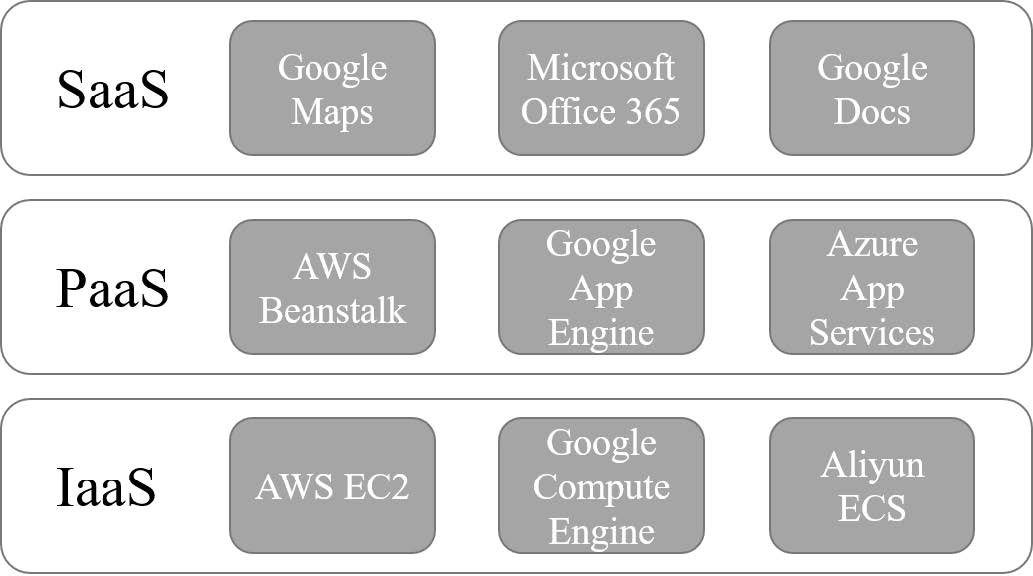
\includegraphics[width=\textwidth]{figures/rep_products.jpg}}
    \caption{云计算服务模型代表产品}
    \label{rep_products}
\end{figure}

% vim:ts=4:sw=4
